\documentclass[12pt, letterpaper]{article}
\usepackage[utf8]{inputenc}
\usepackage[margin=1in]{geometry}
\usepackage{amsmath}
\usepackage{amssymb}
\usepackage{fancyhdr}
\usepackage{pgfplots}
\usepackage{graphicx}
\usepackage{mathtools}
\pgfplotsset{compat=1.16}
\graphicspath{ {./pictures/} }

\title{Portofolio Assignment 1}
\author{Candidate: 25}
\date{September 2020}

\pagestyle{fancy}
\renewcommand{\headrulewidth}{0pt}
\renewcommand{\footrulewidth}{0pt}

\fancyhf{}
\rhead{
    candidate: 25\\
}
\rfoot{Page \thepage}

\begin{document}
  \maketitle
  \section*{Problem 1}
    \subsection*{(1a)} \\
      Supervised learning consists of machine learning algorithms which both has inputs and outputs. The goal of the supervised learning algorithm is using the observed values of $x$ to make an prediction of $y$, where we, the creater of the algorithm is the supervisor. So generally the algorithm consists of whats called a mapping of $x$ to $y$. Or we can generalize this as $y = f(x)$, where $f$ is the mapping of $x$ to $y$. Examples of supervised learning algorithms include classification, regression etc.\\
      \newline
      Whereas in unsupervised learning the goal of the algorithm is to find connections in the data, such that we can learn more from it. Here we don't have a supervisor, we simply try to better see patterns in the input data. We also aren't interested in any output since the input is used to train the model to rule out differences of the variables.\\
      \newline
      The PageRank algorithm is a unsupervised learning algorithm.

      \newline



    \subsection*{(1b)}
      We are given an equation representing the PageRank method,
      \begin{align} \label{eq1}
        r(P_i) = \sum\limits_{P_j \in B_{P_i}} \dfrac{r(P_j)}{|P_j|}.
      \end{align}
      This sum ranks, with the $r(P_i)$ method, the given page, where $p_1, p_2, ... , p_n$ represent all the pages we want to compare against, where $n$ is the number of pages. $P_j$ is a page contained within the set of all the other pages that links to $P_i$, denoted $B_{P_i}$. Then the same is true for $r(P_j)$ as is for $r(P_i)$. $|P_j|$ represents the number of links from $P_j$ to other pages.\\
      \newline
      This equation will provide a ranking vector, $\pi$, to all the pages $p_1,...,p_n$. That means we need $n$ of these rankings to compute all the ranks for the different pages.\\
      In a sense we can view this as a way for each page to cast a \textit{vote} for the other pages, but it's altered in a way that we can see in equation \ref{eq1}. What happens here is that to give a rank to page $i$, we sum all the ranks of the other pages that link to page $i$, and divide each of those pages rank by their outlinks. If we now say again that each page can cast a vote for another page, then the rank gained by page $i$ from a particular page $j$ is the vote, divided by the other votes page $j$ has casted to other pages.
    \subsection*{(1c)}
      For this problem I'll show an example i think makes everything a bit clearer.\\
      \quad We are given 3 pages: $P_1, P_2, P_3$
      \begin{figure}[h]
        \caption{Illustration of the example}
        \centering
        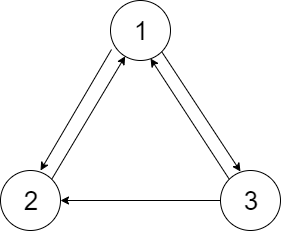
\includegraphics[width=6cm, height=5cm]{Page}
      \end{figure}
      \newline
      This system gives the transitionmatrix, $H^T = $
      \begin{bmatrix}
        0 & 1 & 1/2\\
        1/2 & 0 & 1/2\\
        1/2 & 0 & 0
      \end{bmatrix}
      . \\Where the first column represents $P_1$'s votes for $P_2$ and $P_3$. We note that $P_1$'s votes have been divided by the total number of votes $P_1$ has given. This also goes for the second and third column. This means if we write this as equation \ref{eq1} we get the system:\\
      \begin{align*}
        r(P_1) & = \dfrac{r(P_1)}{|P_1|} + \dfrac{r(P_2)}{|P_2|} + \dfrac{r(P_3)}{|P_3|} \\
        r(P_2) & = \dfrac{r(P_1)}{|P_1|} + \dfrac{r(P_2)}{|P_2|} + \dfrac{r(P_3)}{|P_3|} \\
        r(P_3) & = \dfrac{r(P_1)}{|P_1|} + \dfrac{r(P_2)}{|P_2|} + \dfrac{r(P_3)}{|P_3|}
      \end{align*}
      Which look suspiciously similar to a matrix system of equations.
      Let's define a vector $\pi$, such that, \\
      \vskip0.5cm
      $\pi = $\begin{bmatrix}
        r(P_1)\\
        r(P_2)\\
        r(P_3)
      \end{bmatrix}
      , then when we calculate $H^T \pi$\\
      We get, $H^T \pi = $
      \begin{bmatrix}
        r(P_2) + \dfrac{r(P_3)}{2} \\ \dfrac{r(P_1)}{2} + \dfrac{r(P_3)}{2} \\ \dfrac{r(P_1)}{2}
      \end{bmatrix}
      $=$
      \begin{bmatrix}
        r(P_1)\\r(P_2)\\r(P_3)
      \end{bmatrix}
      $ = \pi \quad(\Rightarrow \lambda = 1)$\\
      Which is our eigenvector. This also holds for the general case with $n$ pages.\\
      To solve this as an iterative method we use the power method. The power method consists of a random vector, that sums to one, which means it's normalized. Then if you multiply the matrix by itself many times, the transition matrix will converge. The remaining step now is to multiply the random vector with the \textit{power matrix}, to get an eigenvector, hence the name power method. Because of the convergent behavior of the transition matrix we know that we will always get the same eigenvector as an result of the multiplication.\\
    \subsection*{(1d)}
      If a matrix is stochastic that means that every element of a matrix $A$, with elements, $[a_{ij}]$ has the property $0 \leq a_{ij} \leq 1$, where each row sums to $1$. This can also be seen in the matrix i wrote in the example of the previous task, $H^T$. Here we see that each row of $H$ sums to $1$, since each row of $H$ represents page $i$ casting votes which is divided by the sum of the row.\\
      \newline
      The irreducability of a matrix basically just means that if we imagine being on a page, we have the possibility to travel to any other pages. We do this by adding a slight and equal portion to all elements which are zero. This we do to prevent \textit{danglin-nodes} which means to prevent you traveling from one page to anthor which does not have another outlink. In my code i used the Google matrix which i had implemented from earlier. This approach does this by adding a small value to all elements of the matrix.
    \subsection*{(1e)}
      We have:
      \begin{align} \label{eq2}
        a_{ij} = \dfrac{L_{ij}}{\sum_{k=1}^{n}L_{ik}}
      \end{align}
      From equation \ref{eq2} we see that the matrix is stochastic, since a value at $ij$ would be the same as a outlink in our conventional manner, then it is divided by the sum of the row. This matrix will however not be irreducable, since there obviously exist dangling nodes with this approach.
    \subsection*{(1g)}
      The main difference is that all dangling nodes are gone. Also many of the players which had previously had the same rank are now instead ranked in relation to each other.
    \subsection*{(1h)}
      From my implementation of the linear regression model we get back two paramaters, $\beta_0, \beta_1$. Where $\beta_0$ is the y-intercept, meaning where the regression line crosses the y-axis. While $\beta_1$ on the other hand is the slope of the regression line. Meaning that in this system we have $y = \beta_1 \cdot x + \beta_0$, where $x$ is our $ln(PageRank)$, and $y$ the Elo-rating.
    \subsection*{(1i)}
      We see that we get a $R^2$-value of $0.721$ which is a measure of how well our regression line fit the given data. While mean squared error is the mean of the error, that is, the distance between the regression line and the actual Elo-rank.\\
      \begin{figure}[h]
        \caption{Comparison between logarithmic and non-logarithmic linear model}
        \centering
        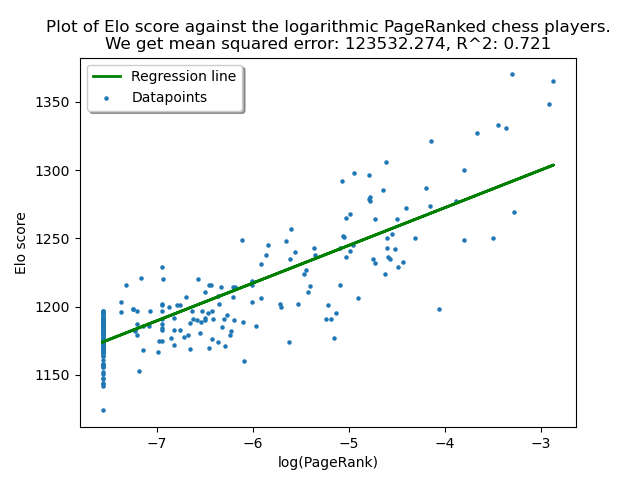
\includegraphics[width=8cm, height=7cm]{logarithmic}
        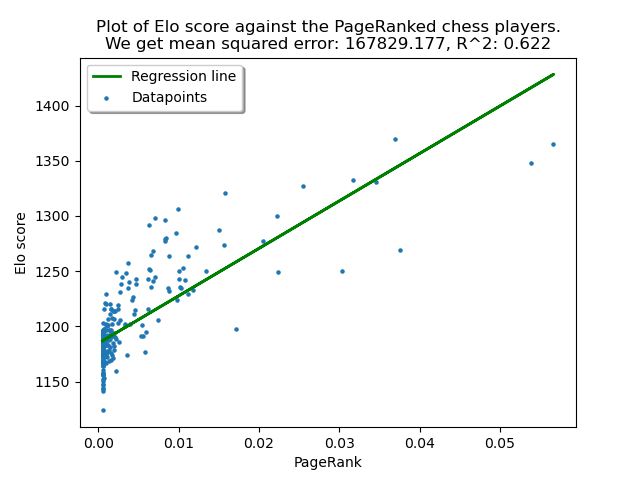
\includegraphics[width=8cm, height=7cm]{nonlogarithmic}
      \end{figure}\\
      What we see here is that with the logarithmic model we get a higher $R^2$ value, and a lower mean squared error which both are better in the logarithmic case than in the non logarithmic case. Taking the $R^2$ value into consideration we could say the logarithmic model is a $9.9$ percent better fit.
  \newpage
  \section*{Problem2}
    \subsection*{(2a)}
      We are to show that the Maximum Likelihood estimators for the unknown parameters.
      \begin{align*}
        p(x|C_0) & = \dfrac{1}{\beta^\alpha\Gamma(\alpha)}x^{\lpha-1}e^{-x/\beta}
        = \
      \end{align*}


\end{document}
